\section{Experiments}
\label{sec:experiments}

\noindent\textbf{Status.} All numbers are independent runs from this repository
(\texttt{experiments/}), on the subsets named below. The general 40-root QPEP solver is not
implemented, the GPU leg of the $4\times4$ probe is blocked, BPnP/Pyatov/POLI are out of scope for
3D--3D, and the 54-scene 3DMatch \emph{training} corpus is not used (all eight official \emph{test}
scenes are covered).

\subsection{Scope and evaluation protocol}

The task is 3D--3D registration with residual
$\mathbf{r}_i=R(\mathbf{q})\mathbf{p}_i+\mathbf{t}-\mathbf{y}_i$, GM kernel with $c=0.05$~m unless
stated, and success $=$ rotation error $<5^\circ$ and translation error $<0.1$~m. RANSAC uses
3-point samples and threshold $\|\mathbf{r}_i\|<c$; the \emph{fixed} baseline always spends 1000
iterations (the v0 protocol), the \emph{adaptive} one uses the standard 0.999 confidence bound capped
at 1000. Unless stated otherwise each cell has 50--100 trials and fixed seeds; runtimes are
single-call wall-clock p50/p95 on a shared CPU node, so speedups are within-run ratios. Wilson $95\%$
lower bounds are $96.3\%$, $97.7\%$, $94.0\%$, and $91.2\%$ for the 100-, 160-, 60-, and 40-trial
cells, so ``100\%'' is not an exact rate. The forward solver is weighted Kabsch, the closed-form
scalar-weight 3D--3D specialization of QPEP; it isolates the robust estimator and the backward, not
the full QPEP algebra, and \textbf{no 40-root QPEP solver is implemented} (a $4\times4$
Davenport/Horn variant is benchmarked in Appendix~\ref{app:systems}).

\subsection{Synthetic forward robustness and cost}

\begin{table}[t]
\caption{Synthetic 3D--3D success rate (\%) under \emph{random} outliers, $N=100$,
100 trials/cell. RANSAC budgets are named: fixed = 1000 iterations, adaptive = 0.999 confidence
cap 1000. Source: \texttt{synthetic/results/main\_table\_extended.json}.}
\label{tab:synthetic}
\centering
\footnotesize
\setlength{\tabcolsep}{3.2pt}
\begin{tabular}{lccccc}
\toprule
$p$ & Kabsch & RANSAC-1000 & RANSAC-adaptive & IRLS-GM & GNC-GM \\
\midrule
0\%  & 100 & 100 & 100 & 100 & 100 \\
10\% & 52  & 100 & 100 & 100 & 100 \\
30\% & 0   & 100 & 100 & 100 & 100 \\
50\% & 0   & 100 & 100 & 100 & 100 \\
70\% & 0   & 100 & 100 & 98  & 100 \\
\bottomrule
\end{tabular}
\end{table}

Table~\ref{tab:synthetic} reports random outliers (replaced observations uniform in $[-2,2]^3$),
100 trials/cell, $N=100$. GNC-GM and both RANSAC variants are at $100\%$ through $70\%$; IRLS drops
to $98\%$ at $70\%$; non-robust Kabsch collapses after $10\%$. Median rotation error is
$0.13$--$0.21^\circ$ for all robust methods; at $p=30\%$ RANSAC-1000 is $0.13^\circ$ and GNC
$0.14^\circ$, tied at two decimals. The meaningful difference is cost: GNC p50 is
$1.48$--$1.63$~ms, RANSAC-1000 $47.7$--$51.9$~ms, adaptive RANSAC $0.41$--$12.36$~ms. Against the
fixed v0 baseline GNC is $\mathbf{31.6}$--$\mathbf{32.5\times}$ faster for $p\ge10\%$; against
adaptive RANSAC it is slower at low $p$ ($3.9\times$ at $10\%$), at parity at $40\%$ ($1.0\times$),
and $8.3\times$ faster at $70\%$ ($25$--$30\times$ at $80$--$90\%$, where adaptive RANSAC saturates
at its cap). RANSAC is not differentiable; GNC's backward is a $6\times6$ solve. LO-RANSAC ties
accuracy but is itself $1.03$--$1.52\times$ slower than adaptive RANSAC
(Appendix~\ref{app:ablations}), so the fixed-1000 baseline is a strawman for runtime; the honest
statement is ``GNC is $22$--$32\times$ faster than fixed-budget RANSAC and has flat runtime at high
outlier rates'', not ``faster than all RANSAC''.

Random outliers flatter every method. A finer breakdown sweep (100--200 trials/cell) shows the
RANSAC failure at $80$--$90\%$: at $90\%$ random outliers RANSAC-1000 is $51\%$, GNC $62\%$, IRLS
$32\%$; at $80\%$ GNC is $89\%$ while RANSAC is $100\%$. With one coherent competing rigid
transform all methods are at $100\%$ through $45\%$ and then collapse: at $50\%$ GNC is $52\%$ and
RANSAC $50\%$, at $55\%$ GNC $2.5\%$ and RANSAC $0\%$, and at $60\%$ every method returns the
\emph{outlier} transform ($100\%$ recovered-outlier rate). This is the identifiability failure of
Section~\ref{sec:discussion}, not a solver bug. With boundary outliers ($e/c^2\sim U(1/3,3)$) all
methods remain at $100\%$ even at $70\%$, and the robust methods are more accurate (GNC
$0.27^\circ$ vs RANSAC $0.62^\circ$ and Kabsch $0.33^\circ$ at $70\%$); forward success is not
where boundary outliers bite.

\subsection{Exact gradient versus frozen weights}

The 6D gradient table uses $N=30$, ten $40\%$-boundary and ten $20\%$-random instances, GNC plus
Newton polish to $\|\Phi\|\sim10^{-13}$, and central finite differences of the polished fixed-point
branch ($h=10^{-5}$). The exact IFT Jacobian matches FD to a relative Frobenius error of
$\mathbf{4.9\times10^{-8}}$ (inliers), $\mathbf{3.1\times10^{-8}}$ (boundary), and
$1.25\times10^{-4}$ (gross, FD-cancellation-limited), with cosine $1.000000$. The naive
frozen-weight Jacobian is $0.212$ (inlier) and $\mathbf{1.07}$ (boundary) relative error, with
boundary cosine $0.234$ (min $-0.358$). Omitting only the $-\lambda_{\mathrm{rob}}$ term gives
$9.0\times10^{-4}$--$9.8\times10^{-4}$ relative error, so the curvature correction is the dominant
missing term, not the constraint term.

\begin{table}[t]
\caption{6D Jacobian versus central finite differences of the polished fixed-point branch
($N=30$). Relative error and cosine are medians unless marked min. $^\ast$FD-cancellation-limited;
the absolute error remains small and the cosine is $1$. Source:
\texttt{synthetic/results/gradient\_table.json}.}
\label{tab:gradient}
\centering
\footnotesize
\setlength{\tabcolsep}{3pt}
\begin{tabular}{llrccc}
\toprule
bin & method & $n$ & rel.\ err p50 & cos p50 & min \\
\midrule
inlier   & exact & 414 & $4.9\times10^{-8}$ & 1.000000 & 1.000000 \\
inlier   & naive & 414 & $2.12\times10^{-1}$ & 0.985 & 0.791 \\
boundary & exact & 122 & $3.1\times10^{-8}$ & 1.000000 & 1.000000 \\
boundary & naive & 122 & $\mathbf{1.07}$ & $\mathbf{0.234}$ & $\mathbf{-0.358}$ \\
gross    & exact & 64  & $1.25\times10^{-4\ast}$ & 1.000000 & 0.9986 \\
gross    & naive & 64  & $1.16$ & $-0.118$ & $-0.397$ \\
\bottomrule
\end{tabular}
\end{table}

For observations with $e>c^2/3$, the mapping-level radial response has the opposite sign for exact
versus naive in $\mathbf{100\%}$ of boundary ($122/122$) and gross ($64/64$) observations; the
pose-translation level also flips in $100\%$ of this well-conditioned 6D sample. The 1D statement is
a theorem (Proposition~\ref{prop:signflip}); the 6D statement remains a numerical observation.

\subsection{End-to-end boundary diagnostic}

A GT-supervised test-time refinement updates only the injected boundary observations for 20 Adam
steps. At $p=0.5$, lr $10^{-3}$, exact reaches a final loss of $1.90\times10^{-6}$ vs
$1.66\times10^{-5}$ for naive (paired median ratio $0.071$, a $14\times$ reduction; exact lower on
$10/10$ seeds) and rotation error $0.029^\circ$ vs $0.087^\circ$. At $p=0.7$ the paired median ratio
is $0.059$ ($17\times$) and exact wins $9/10$. The all-points control is not discriminative
($4$--$9/10$, ratio $0.64$--$1.04$). The gradient check is exact to $1.6\times10^{-7}$ /
$3.9\times10^{-8}$ / $9.3\times10^{-8}$ relative error per coordinate; naive is $1.42$ / $0.60$ /
$0.38$. A float64 PyTorch \texttt{autograd.Function} passes \texttt{gradcheck} at $N=6/8/10$ (max
absolute error $6$--$8\times10^{-10}$; max relative $8\times10^{-9}$--$1.1\times10^{-8}$, except one
near-zero element at $8\times10^{-6}$); the naive backward fails at $1.5$--$1.8$, and the torch port
agrees with NumPy to $10^{-16}$ in pose and $3\times10^{-16}$ in $\mathrm{d}L/\mathrm{d}\mathbf{y}$.
A per-point MLP refinement (5 seeds, $p=0.4$, 50 Adam steps) reduces median rotation from
$0.635^\circ$ to $0.068^\circ$ for exact vs $0.106^\circ$ for naive (exact wins $4/5$ seeds, median
loss ratio $0.56$); a disjoint held-out protocol is \textbf{negative}---both arms overfit. This is a
toy validation, not a trained real-data system.

\subsection{Real geometry}

\begin{table*}[t]
\caption{Measured real-data summary. Success is rotation $<5^\circ$ and translation $<0.1$~m under
random outliers; speedups are GNC-GM p50 over \emph{fixed-1000} RANSAC p50 (adaptive RANSAC is
discussed in the text). ``---'' = not applicable. All rows are independent reproductions from
\texttt{experiments/real/}; per-dataset and per-scene detail, including the GT verification and
window metadata, is in Appendix~\ref{app:datasets}.}
\label{tab:real}
\centering
\footnotesize
\setlength{\tabcolsep}{3.5pt}
\begin{tabular}{llcccc}
\toprule
dataset & measured subset & success & error & speedup vs fixed & note \\
\midrule
3DMatch & all 8 official test scenes, 20 trials/cell & $100\%$ $\le70\%$ & $0.27^\circ$ @$70\%$ bnd &
$27.7\times$ & coherent: $46\%$ vs $3\%$ @$50\%$ \\
KITTI raw & drives 0001/0002 (108/77 frames), 10 pairs & $100\%$ $\le70\%$ &
$0.07$--$0.09^\circ$ @$70\%$ & $\sim22\times$ & bnd: RANSAC $0.14$--$0.16^\circ$ \\
KITTI odom. & all 11 sequences 00--10, 33 frames each & $99/99/100/100\%$ & $0.067^\circ$ @$70\%$ &
$22.4\times$ & seq 08 $80\%$ @$p\le0.3$ \\
In-The-Dark day & 2 runs, 15 pairs each & $100\%$ @$0.1$~m & $0.078$/$0.092^\circ$ & --- &
$0.020$/$0.010$~m; $79.4/88.5\%$ inl. \\
In-The-Dark night & 2 windows, 10 pairs each & $100\%$ @$0.1$~m & $0.135$/$0.150^\circ$ & --- &
$0.011$~m; $96.0/97.1\%$ inl. \\
\bottomrule
\end{tabular}
\end{table*}

\noindent\textbf{ModelNet40/10.} With real object point clouds, 50 trials/cell and uniform outliers,
GNC-GM is $100\%$ at $0$--$70\%$ on both datasets; RANSAC-1000 is $100\%$, IRLS $98$--$100\%$, and
Kabsch collapses at $50\%$. GNC is $1.7$--$1.9$~ms vs $53.5$--$61.5$~ms ($30$--$32.5\times$).
ModelNet10 (908 test objects, 10 classes, 2048 points) differs from ModelNet40 by at most $2$~pp
success and $0.038^\circ$ median rotation.

\noindent\textbf{3DMatch.} All eight official test scenes are processed with the official TSDF
clouds and \texttt{gt.log}, with GT-mapped nearest-neighbour correspondences (oracle matches with
real scan/occlusion residual), $N=300$, $c=0.05$~m, 20 trials/cell, 8 high-overlap pairs/scene.
Random outliers: GNC and RANSAC-1000 are $100\%$ through $70\%$ (IRLS $99\%$ at $70\%$), pooled GNC
p50 $2.26$~ms vs $62.6$~ms ($27.7\times$; per scene $2.26$--$2.36$ vs $62.1$--$73.4$~ms,
$27.4$--$31.1\times$). Coherent outliers collapse at $60$--$70\%$ for every method ($0\%$); at
$50\%$ GNC is $46\%$ and RANSAC $3\%$. The low/mid/high overlap study (24/21/20 pairs) gives clean
rotation $0.52/0.24/0.18^\circ$ with both robust methods at $100\%$ at $p=0.7$ in every bin
(speedup $27.7$--$30.4\times$ for $p\ge30\%$); a stricter $0.20$--$0.50$ geometric-overlap band has
oracle base inlier $0.953$/$0.984$ and clean rotation $0.47^\circ$/$0.19^\circ$, where GNC and
RANSAC remain $100\%$ at $p=0.7$ (IRLS $92\%$, Kabsch $1\%$). A hand-crafted FPFH front-end (no GT
in matching) reaches $80.0\%$/$67.8\%$ natural inliers with GNC $100\%$/$100\%$, RANSAC-1000
$100\%$/$97\%$, Kabsch $100\%$/$83\%$---not FCGF/Predator.

\noindent\textbf{KITTI.} Two raw drives (2011\_09\_26 drives 0001/0002, 108/77 frames) give real
outdoor LiDAR (OXTS motion mapped with \texttt{calib\_imu\_to\_velo}, direction verified). With
$N=300$, $c=0.25$~m, 10 pairs and 20 trials/cell, GNC and RANSAC-1000 are $100\%$ through $70\%$;
GNC p50 is $2.7$--$2.8$~ms vs $61$--$64$~ms ($\sim22\times$), coherent $60$--$70\%$ collapses for
all methods, and boundary is $100\%$ for GNC and IRLS ($0.07$--$0.09^\circ$ vs RANSAC
$0.14$--$0.16^\circ$ at $70\%$). Drive 0002 reproduces the drive-0001 tables and the coherent
transition (at $50\%$ GNC $40\%$ vs $35\%$, IRLS $30\%$ vs $45\%$, both chance-level). For odometry,
all 11 sequences 00--10 are represented by 33 selected frames each (32--33 touched frames
range-fetched from the 84.8~GB archive). On the eight added sequences (10 trials/cell) success is
$100\%$ for GNC and RANSAC-1000 at $p=0.7$ except seq~08, where GNC is $80\%$ at $p=0$ and $p=0.3$
(a real bad-basin failure, RANSAC $100\%$); pooled over 11 sequences success is
$99/99/100/100\%$ at $p=0/0.3/0.5/0.7$ and the fixed-RANSAC/GNC runtime ratio is $22.4\times$ at
$p\ge0.3$. The 00/05/07 subset gives the failure-mode detail: coherent collapse at $p=0.6$ (at
$p=0.5$ GNC $53\%$, IRLS $38\%$, RANSAC $0\%$), boundary $0.067^\circ$ vs $0.143^\circ$, and across
$|\mathbf{t}|=0.09$--$9.62$~m and gaps $1/2/4/8$ (171 paired cells) GNC is never below RANSAC. The
clean floor $0.042$--$0.057^\circ$ is not lower than the OXTS drives ($0.030$--$0.039^\circ$), so
sampling, not pose error, dominates it. The 33 frames per sequence are a subset, not the full
streams.

\noindent\textbf{UTIAS In-The-Dark (day and night prefixes) \cite{utias2020inthedark}.} The
official per-pair GT was composed from repeat spatial $\times$ teach temporal $\times$
camera--vehicle conjugation and validated by stereo reprojection: $0.65$~px (run\_000002) and
$0.52$~px (run\_000012) median vs $18.1/27.9$~px inverse, $9.5/14.7$~px identity, and
$21.5/31.3$~px unconjugated. On 15 consecutive daytime pairs per run with the hand-written
SIFT+StereoSGBM front-end (same \texttt{stereo\_vo.py} as the KITTI fallback, \emph{not} SDPR's
VGG/UNet), natural inliers are $79.4\%$/$88.5\%$ and GNC-GM reaches
$\mathbf{0.078^\circ/0.020}$~m and $\mathbf{0.092^\circ/0.010}$~m with $100\%$ at $0.1$~m (Kabsch
$47\%/40\%$); both runs are morning/sunny. Two night-time windows (run\_000017 at 21:58,
run\_000018 at 22:28), 10 consecutive pairs each: dense SGBM gives $96.0\%$/$97.1\%$ inliers and GNC
$0.135^\circ/0.011$~m and $0.150^\circ/0.011$~m, both $100\%$ at $0.1$~m; sparse night is $84.3\%$
and $0.197^\circ/0.015$~m. A motion-matched daylight control (run\_000002 start 757,
$|\mathbf{t}|=0.21$~m, rot $0.54^\circ$) gives $85.9\%$ inliers and $0.121^\circ/0.007$~m, so the
night inlier advantage is mostly a closer-range/geometry effect (median depth $4.5$~m at night vs
$6.7$--$7.2$~m by day), \textbf{not evidence that SIFT is more robust in the dark}. These are
10-pair windows, not full night runs.

\noindent\textbf{KITTI stereo fallback (negative translation).} A SIFT + sub-pixel + StereoSGBM
front-end on rectified \texttt{image\_02/03} ($b=0.5327$~m), 30 pairs of drive 0001: natural inlier
rate $17.8\%$ at $c=0.5$~m with 890 correspondences/pair. GNC/IRLS recover rotation to $0.052^\circ$
(GT-inlier floor $0.071^\circ$), but translation is $0.70$~m median vs $1.92$~m motion and a
$0.239$~m floor; \textbf{no method reaches $0.1$~m or $0.25$~m}. GNC is $19.3\times$ faster than
fixed RANSAC (4.21 vs 81.3~ms). A stereo-vs-LiDAR depth ratio of $1.000$--$1.061$ over 3--60~m
rules out a disparity-scale bug; the residual is a coherent forward-translation under-estimate
($0.63$--$0.73$). The layer solves rotation but cannot repair a biased front-end.

\subsection{Systems, baselines, and ablations}

A vectorized numpy GNC over $(B,N,3)$ reproduces the loop to $1.1\times10^{-14}$ (rotation) and
$1.2\times10^{-15}$ (translation); at $B=32,N=100$ batch p50 is $8.5$~ms vs $56.2$~ms
($6.60\times$), $B=8$ gives $2.95\times$/$3.27\times$, and $B=1$ is slower ($0.54\times$). On an RTX
5090 the float64 eager torch launch floor is $42.4$--$45.7$~ms: GPU loses at $B\le8$
($0.04$--$0.57\times$), ties at $B=32,N=100$ ($1.33\times$), and wins at $B=32,N=500$
($2.23\times$) and $B=128$ ($4.96\times$/$8.24\times$). The $4\times4$ Davenport/Horn inner solver
\cite{horn1987} is numerically equivalent to weighted Kabsch (max $\|R_d-R_k\|_F=1.07\times10^{-14}$,
cost excess $9.4\times10^{-16}$) but faster only at large $N$. On synthetic data, Theseus 0.2.3
(dense Cholesky; Jacobian vs FD $1.09\times10^{-10}$) with GT initialization succeeds $100\%$ at
all $p$ (local-basin check) and with random initialization $100/80/55/25\%$ at $p=0/0.3/0.5/0.7$ at
$358$--$670$~ms, while GNC-GM is $100\%$ at $1.7$~ms on the same 20 instances (the $p=0.3$ Wilson
intervals overlap). SDPRLayers+SCS is numerically available ($0/208$ exceptions, $8.5$--$13.4$~ms)
but succeeds only at $p=0$, as expected without a robust kernel; with $W_i=I$ its objective equals
Kabsch (80 paired trials, max $|\Delta R|=1.5\times10^{-5}$~deg, max $|\Delta t|=1.3\times10^{-9}$~m),
so it is a forward-correctness check, \emph{not} a robust baseline. \textbf{BPnP, Pyatov \emph{et
al.}, and POLI were not run} (3D--2D PnP, two-view 2D--2D, and a geometry estimator with no official
pose-solver code, respectively), so no 3D--3D table is fabricated. Kernel, schedule, RANSAC-strength,
and anisotropic-weight ablations are in Appendix~\ref{app:ablations}.

\subsection{What is not measured}
\label{sec:notmeasured}

\textbf{Not claimed}: (i) external baselines are synthetic-only (SDPRLayers is forward-only with
SCS, no Mosek; Theseus uses dense Cholesky); (ii) In-The-Dark is two daylight runs (15 pairs each)
plus two night \emph{windows} (10 pairs each), with a hand-written SIFT+SGBM front-end, not SDPR's
VGG/UNet, and no training---full night runs, glare/headlight extremes, and end-to-end training are
untested; (iii) no learned descriptors (the only descriptor front-end is hand-crafted FPFH); (iv) the
54-scene 3DMatch \emph{training} corpus is not used, and the true $0.20$--$0.50$ geometric-overlap
band still has oracle base inlier $0.88$--$0.99$; KITTI odometry 00--10 is 33 selected frames per
sequence, not the full streams; (v) the 40-root QPEP polynomial solver, its root completeness, and
GPU batching of it---the GPU probe covers only the $4\times4$ eigen inner and its GPU leg is
\textbf{blocked by node occupancy} (job 3184 was PENDING with a 21~h estimate and was cancelled; CPU
validation only); (vi) anisotropic $W_i$ under matched noise covariance; (vii) a 6D sign-flip
theorem (numerical); (viii) global optimality, a breakdown-point guarantee, or adversarial
robustness. The coherent-majority failure and the RANSAC-adaptive comparison are reported because
they weaken the strongest possible claims.

\subsection{Falsifiers}
\label{sec:falsify}

Each measured claim is stated so that it can fail; Appendix~\ref{app:falsifiers} lists the
falsifiers and current values (e.g.\ an exact-vs-FD relative error above $10^{-6}$ or a cosine below
$0.999$ would falsify the exact-backward claim; a GNC success below fixed-budget RANSAC at any
$p\in[0,0.7]$ on random outliers would falsify parity).

\begin{figure*}[t]
\centering
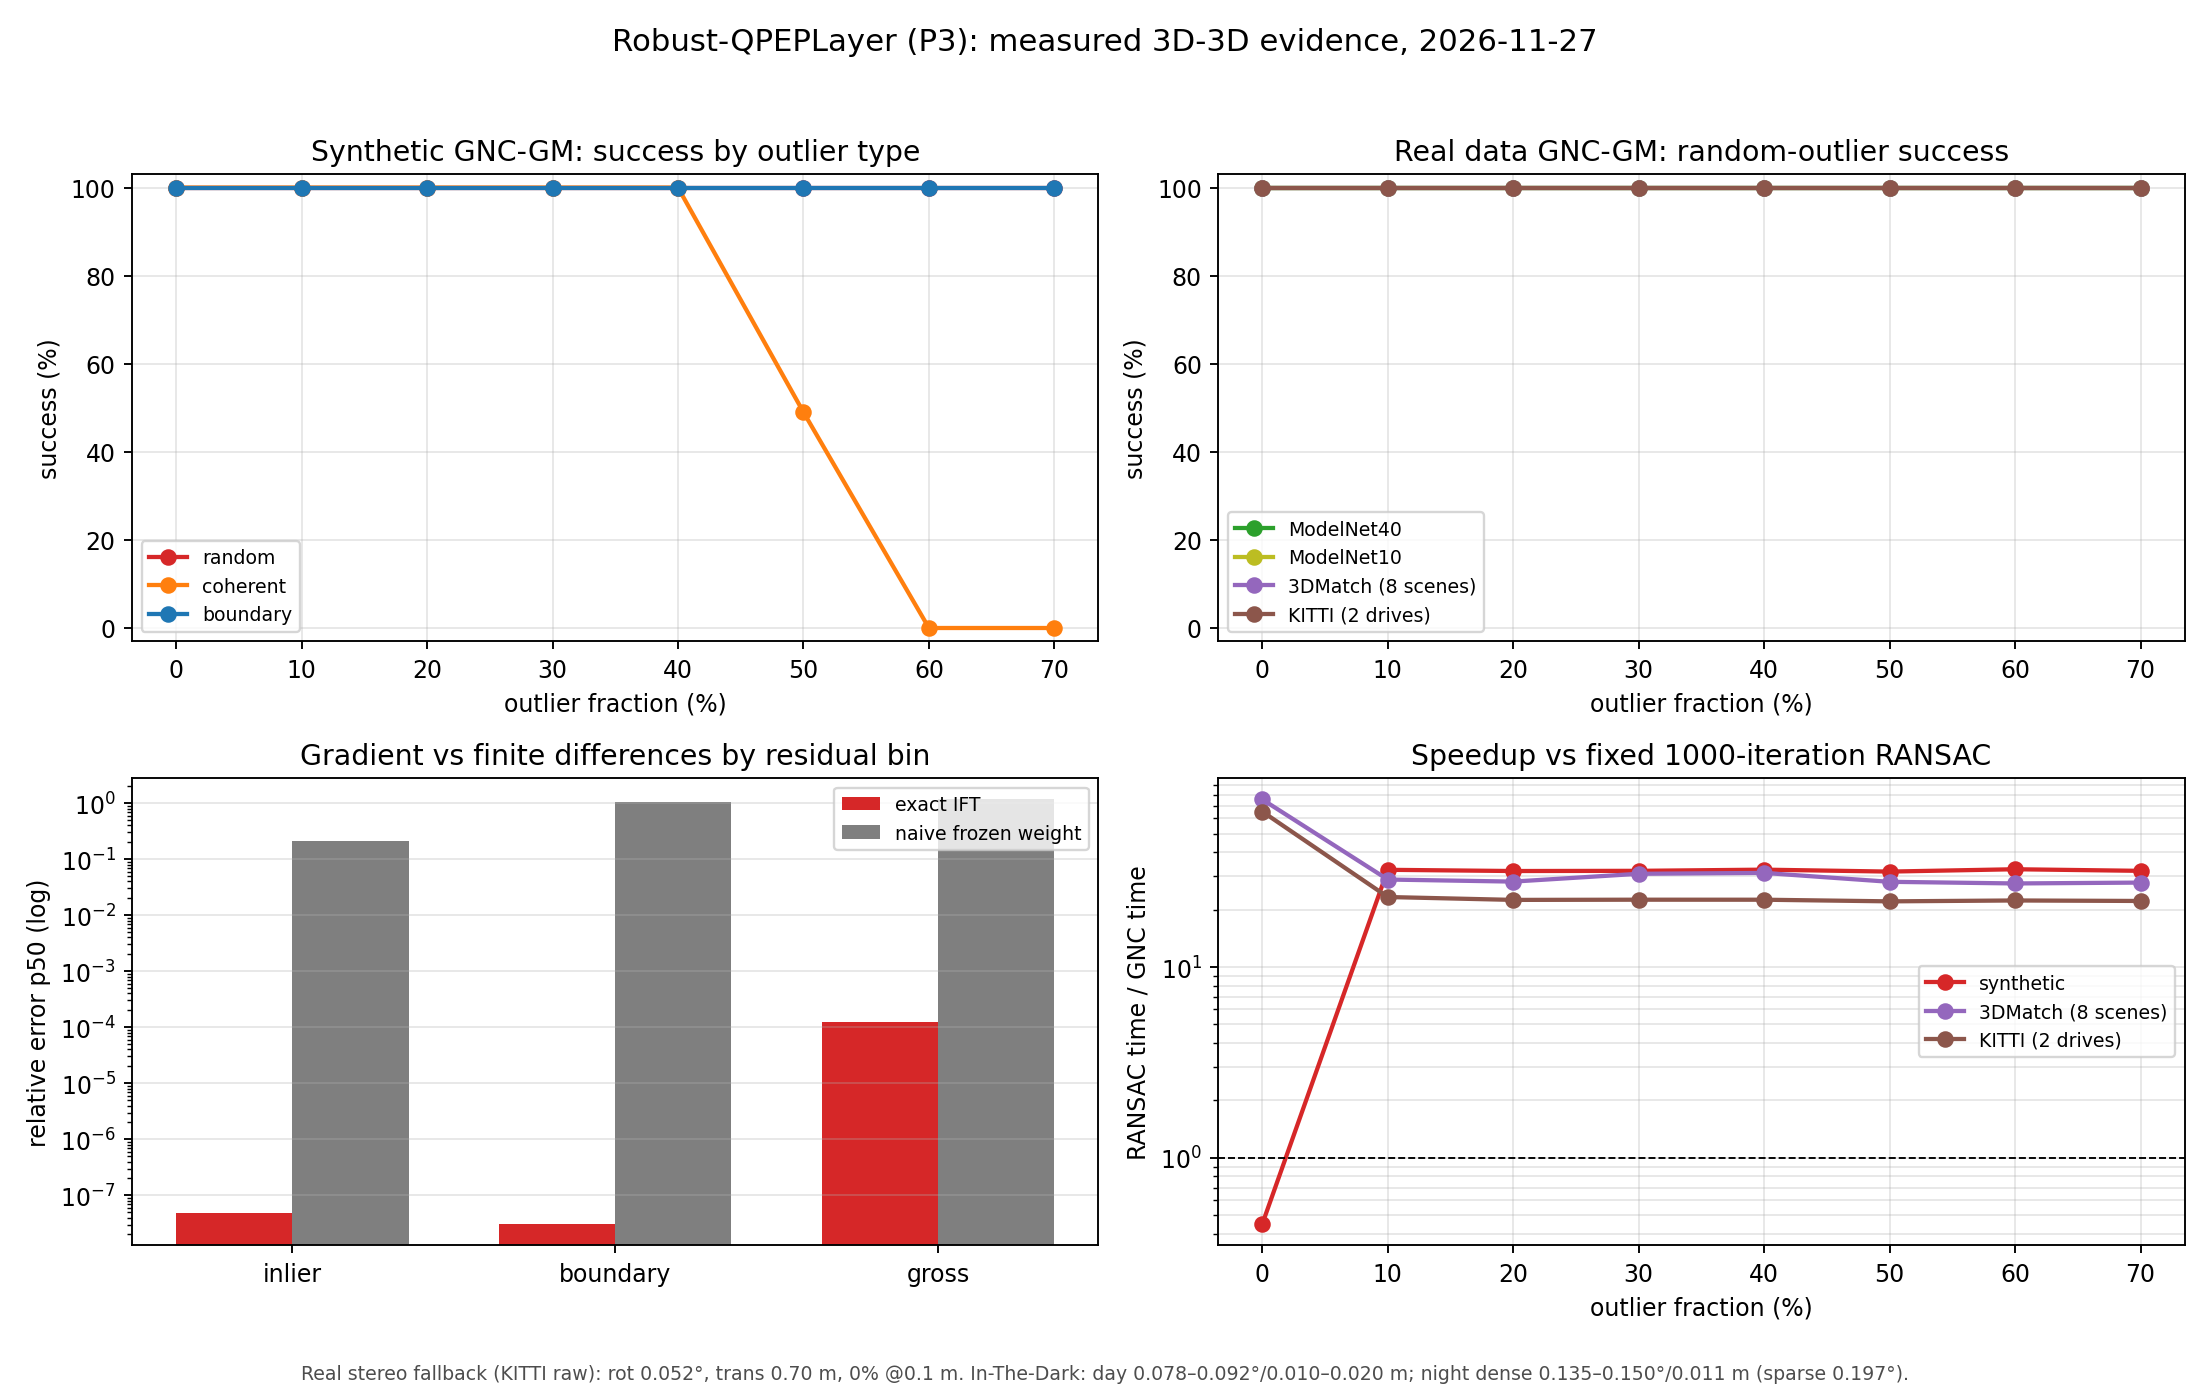
\includegraphics[width=\textwidth]{p3_summary.png}
\caption{Measured 3D--3D evidence (2026-11-27). (a) Synthetic GNC-GM success versus outlier
fraction for random, coherent, and boundary outliers: random and boundary stay at $100\%$,
coherent collapses once the outlier transform becomes the global optimum. (b) Real-data
random-outlier success for ModelNet40, ModelNet10, 3DMatch (8 scenes), and KITTI (2 drives); all
stay at $100\%$ through $70\%$. (c) 6D Jacobian relative error (p50, log scale) of exact IFT
versus naive frozen weights, by residual bin; the boundary bin is where freezing fails. (d)
GNC p50 runtime advantage over \emph{fixed-1000} RANSAC on synthetic, 3DMatch, and KITTI data; the
dashed line is break-even. The footer reports the KITTI stereo fallback and the In-The-Dark
day/night ranges. Success is rotation $<5^\circ$ and translation $<0.1$~m; source:
\texttt{experiments/make\_summary\_figure.py}.}
\label{fig:summary}
\end{figure*}
